% Created by tikzDevice version 0.10.1 on 2016-08-19 15:24:06
% !TEX encoding = UTF-8 Unicode
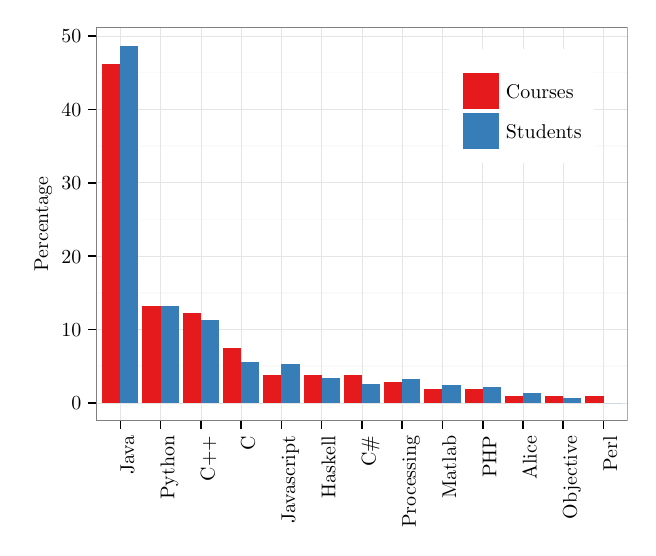
\begin{tikzpicture}[x=1pt,y=1pt]
\definecolor{fillColor}{RGB}{255,255,255}
\path[use as bounding box,fill=fillColor,fill opacity=0.00] (0,0) rectangle (216.81,180.67);
\begin{scope}
\path[clip] (  0.00,  0.00) rectangle (216.81,180.67);
\definecolor{drawColor}{RGB}{255,255,255}
\definecolor{fillColor}{RGB}{255,255,255}

\path[draw=drawColor,line width= 0.6pt,line join=round,line cap=round,fill=fillColor] (  0.00,  0.00) rectangle (216.81,180.68);
\end{scope}
\begin{scope}
\path[clip] ( 24.76, 38.59) rectangle (216.81,180.67);
\definecolor{fillColor}{RGB}{255,255,255}

\path[fill=fillColor] ( 24.76, 38.59) rectangle (216.81,180.67);
\definecolor{drawColor}{gray}{0.98}

\path[draw=drawColor,line width= 0.6pt,line join=round] ( 24.76, 58.31) --
	(216.81, 58.31);

\path[draw=drawColor,line width= 0.6pt,line join=round] ( 24.76, 84.84) --
	(216.81, 84.84);

\path[draw=drawColor,line width= 0.6pt,line join=round] ( 24.76,111.36) --
	(216.81,111.36);

\path[draw=drawColor,line width= 0.6pt,line join=round] ( 24.76,137.89) --
	(216.81,137.89);

\path[draw=drawColor,line width= 0.6pt,line join=round] ( 24.76,164.41) --
	(216.81,164.41);
\definecolor{drawColor}{gray}{0.90}

\path[draw=drawColor,line width= 0.2pt,line join=round] ( 24.76, 45.05) --
	(216.81, 45.05);

\path[draw=drawColor,line width= 0.2pt,line join=round] ( 24.76, 71.58) --
	(216.81, 71.58);

\path[draw=drawColor,line width= 0.2pt,line join=round] ( 24.76, 98.10) --
	(216.81, 98.10);

\path[draw=drawColor,line width= 0.2pt,line join=round] ( 24.76,124.63) --
	(216.81,124.63);

\path[draw=drawColor,line width= 0.2pt,line join=round] ( 24.76,151.15) --
	(216.81,151.15);

\path[draw=drawColor,line width= 0.2pt,line join=round] ( 24.76,177.68) --
	(216.81,177.68);

\path[draw=drawColor,line width= 0.2pt,line join=round] ( 33.49, 38.59) --
	( 33.49,180.67);

\path[draw=drawColor,line width= 0.2pt,line join=round] ( 48.04, 38.59) --
	( 48.04,180.67);

\path[draw=drawColor,line width= 0.2pt,line join=round] ( 62.59, 38.59) --
	( 62.59,180.67);

\path[draw=drawColor,line width= 0.2pt,line join=round] ( 77.14, 38.59) --
	( 77.14,180.67);

\path[draw=drawColor,line width= 0.2pt,line join=round] ( 91.68, 38.59) --
	( 91.68,180.67);

\path[draw=drawColor,line width= 0.2pt,line join=round] (106.23, 38.59) --
	(106.23,180.67);

\path[draw=drawColor,line width= 0.2pt,line join=round] (120.78, 38.59) --
	(120.78,180.67);

\path[draw=drawColor,line width= 0.2pt,line join=round] (135.33, 38.59) --
	(135.33,180.67);

\path[draw=drawColor,line width= 0.2pt,line join=round] (149.88, 38.59) --
	(149.88,180.67);

\path[draw=drawColor,line width= 0.2pt,line join=round] (164.43, 38.59) --
	(164.43,180.67);

\path[draw=drawColor,line width= 0.2pt,line join=round] (178.98, 38.59) --
	(178.98,180.67);

\path[draw=drawColor,line width= 0.2pt,line join=round] (193.53, 38.59) --
	(193.53,180.67);

\path[draw=drawColor,line width= 0.2pt,line join=round] (208.08, 38.59) --
	(208.08,180.67);
\definecolor{fillColor}{RGB}{228,26,28}

\path[fill=fillColor] ( 26.94, 45.05) rectangle ( 33.49,167.67);
\definecolor{fillColor}{RGB}{55,126,184}

\path[fill=fillColor] ( 33.49, 45.05) rectangle ( 40.03,174.22);
\definecolor{fillColor}{RGB}{228,26,28}

\path[fill=fillColor] ( 41.49, 45.05) rectangle ( 48.04, 80.08);
\definecolor{fillColor}{RGB}{55,126,184}

\path[fill=fillColor] ( 48.04, 45.05) rectangle ( 54.58, 80.16);
\definecolor{fillColor}{RGB}{228,26,28}

\path[fill=fillColor] ( 56.04, 45.05) rectangle ( 62.59, 77.58);
\definecolor{fillColor}{RGB}{55,126,184}

\path[fill=fillColor] ( 62.59, 45.05) rectangle ( 69.13, 75.17);
\definecolor{fillColor}{RGB}{228,26,28}

\path[fill=fillColor] ( 70.59, 45.05) rectangle ( 77.14, 65.07);
\definecolor{fillColor}{RGB}{55,126,184}

\path[fill=fillColor] ( 77.14, 45.05) rectangle ( 83.68, 59.82);
\definecolor{fillColor}{RGB}{228,26,28}

\path[fill=fillColor] ( 85.14, 45.05) rectangle ( 91.68, 55.06);
\definecolor{fillColor}{RGB}{55,126,184}

\path[fill=fillColor] ( 91.68, 45.05) rectangle ( 98.23, 59.15);
\definecolor{fillColor}{RGB}{228,26,28}

\path[fill=fillColor] ( 99.69, 45.05) rectangle (106.23, 55.06);
\definecolor{fillColor}{RGB}{55,126,184}

\path[fill=fillColor] (106.23, 45.05) rectangle (112.78, 54.18);
\definecolor{fillColor}{RGB}{228,26,28}

\path[fill=fillColor] (114.24, 45.05) rectangle (120.78, 55.06);
\definecolor{fillColor}{RGB}{55,126,184}

\path[fill=fillColor] (120.78, 45.05) rectangle (127.33, 51.78);
\definecolor{fillColor}{RGB}{228,26,28}

\path[fill=fillColor] (128.79, 45.05) rectangle (135.33, 52.56);
\definecolor{fillColor}{RGB}{55,126,184}

\path[fill=fillColor] (135.33, 45.05) rectangle (141.88, 53.59);
\definecolor{fillColor}{RGB}{228,26,28}

\path[fill=fillColor] (143.34, 45.05) rectangle (149.88, 50.06);
\definecolor{fillColor}{RGB}{55,126,184}

\path[fill=fillColor] (149.88, 45.05) rectangle (156.43, 51.43);
\definecolor{fillColor}{RGB}{228,26,28}

\path[fill=fillColor] (157.88, 45.05) rectangle (164.43, 50.06);
\definecolor{fillColor}{RGB}{55,126,184}

\path[fill=fillColor] (164.43, 45.05) rectangle (170.98, 50.69);
\definecolor{fillColor}{RGB}{228,26,28}

\path[fill=fillColor] (172.43, 45.05) rectangle (178.98, 47.55);
\definecolor{fillColor}{RGB}{55,126,184}

\path[fill=fillColor] (178.98, 45.05) rectangle (185.53, 48.67);
\definecolor{fillColor}{RGB}{228,26,28}

\path[fill=fillColor] (186.98, 45.05) rectangle (193.53, 47.55);
\definecolor{fillColor}{RGB}{55,126,184}

\path[fill=fillColor] (193.53, 45.05) rectangle (200.08, 46.98);
\definecolor{fillColor}{RGB}{228,26,28}

\path[fill=fillColor] (201.53, 45.05) rectangle (208.08, 47.55);
\definecolor{fillColor}{RGB}{55,126,184}

\path[fill=fillColor] (208.08, 45.05) rectangle (214.63, 45.05);
\definecolor{drawColor}{gray}{0.50}

\path[draw=drawColor,line width= 0.6pt,line join=round,line cap=round] ( 24.76, 38.59) rectangle (216.81,180.67);
\end{scope}
\begin{scope}
\path[clip] (  0.00,  0.00) rectangle (216.81,180.67);
\definecolor{drawColor}{RGB}{0,0,0}

\node[text=drawColor,anchor=base east,inner sep=0pt, outer sep=0pt, scale=  0.72] at ( 19.36, 42.57) {0};

\node[text=drawColor,anchor=base east,inner sep=0pt, outer sep=0pt, scale=  0.72] at ( 19.36, 69.10) {10};

\node[text=drawColor,anchor=base east,inner sep=0pt, outer sep=0pt, scale=  0.72] at ( 19.36, 95.62) {20};

\node[text=drawColor,anchor=base east,inner sep=0pt, outer sep=0pt, scale=  0.72] at ( 19.36,122.15) {30};

\node[text=drawColor,anchor=base east,inner sep=0pt, outer sep=0pt, scale=  0.72] at ( 19.36,148.67) {40};

\node[text=drawColor,anchor=base east,inner sep=0pt, outer sep=0pt, scale=  0.72] at ( 19.36,175.20) {50};
\end{scope}
\begin{scope}
\path[clip] (  0.00,  0.00) rectangle (216.81,180.67);
\definecolor{drawColor}{RGB}{0,0,0}

\path[draw=drawColor,line width= 0.6pt,line join=round] ( 21.76, 45.05) --
	( 24.76, 45.05);

\path[draw=drawColor,line width= 0.6pt,line join=round] ( 21.76, 71.58) --
	( 24.76, 71.58);

\path[draw=drawColor,line width= 0.6pt,line join=round] ( 21.76, 98.10) --
	( 24.76, 98.10);

\path[draw=drawColor,line width= 0.6pt,line join=round] ( 21.76,124.63) --
	( 24.76,124.63);

\path[draw=drawColor,line width= 0.6pt,line join=round] ( 21.76,151.15) --
	( 24.76,151.15);

\path[draw=drawColor,line width= 0.6pt,line join=round] ( 21.76,177.68) --
	( 24.76,177.68);
\end{scope}
\begin{scope}
\path[clip] (  0.00,  0.00) rectangle (216.81,180.67);
\definecolor{drawColor}{RGB}{0,0,0}

\path[draw=drawColor,line width= 0.6pt,line join=round] ( 33.49, 35.59) --
	( 33.49, 38.59);

\path[draw=drawColor,line width= 0.6pt,line join=round] ( 48.04, 35.59) --
	( 48.04, 38.59);

\path[draw=drawColor,line width= 0.6pt,line join=round] ( 62.59, 35.59) --
	( 62.59, 38.59);

\path[draw=drawColor,line width= 0.6pt,line join=round] ( 77.14, 35.59) --
	( 77.14, 38.59);

\path[draw=drawColor,line width= 0.6pt,line join=round] ( 91.68, 35.59) --
	( 91.68, 38.59);

\path[draw=drawColor,line width= 0.6pt,line join=round] (106.23, 35.59) --
	(106.23, 38.59);

\path[draw=drawColor,line width= 0.6pt,line join=round] (120.78, 35.59) --
	(120.78, 38.59);

\path[draw=drawColor,line width= 0.6pt,line join=round] (135.33, 35.59) --
	(135.33, 38.59);

\path[draw=drawColor,line width= 0.6pt,line join=round] (149.88, 35.59) --
	(149.88, 38.59);

\path[draw=drawColor,line width= 0.6pt,line join=round] (164.43, 35.59) --
	(164.43, 38.59);

\path[draw=drawColor,line width= 0.6pt,line join=round] (178.98, 35.59) --
	(178.98, 38.59);

\path[draw=drawColor,line width= 0.6pt,line join=round] (193.53, 35.59) --
	(193.53, 38.59);

\path[draw=drawColor,line width= 0.6pt,line join=round] (208.08, 35.59) --
	(208.08, 38.59);
\end{scope}
\begin{scope}
\path[clip] (  0.00,  0.00) rectangle (216.81,180.67);
\definecolor{drawColor}{RGB}{0,0,0}

\node[text=drawColor,rotate= 90.00,anchor=base east,inner sep=0pt, outer sep=0pt, scale=  0.72] at ( 38.45, 33.19) {Java};

\node[text=drawColor,rotate= 90.00,anchor=base east,inner sep=0pt, outer sep=0pt, scale=  0.72] at ( 52.99, 33.19) {Python};

\node[text=drawColor,rotate= 90.00,anchor=base east,inner sep=0pt, outer sep=0pt, scale=  0.72] at ( 67.54, 33.19) {C++};

\node[text=drawColor,rotate= 90.00,anchor=base east,inner sep=0pt, outer sep=0pt, scale=  0.72] at ( 82.09, 33.19) {C};

\node[text=drawColor,rotate= 90.00,anchor=base east,inner sep=0pt, outer sep=0pt, scale=  0.72] at ( 96.64, 33.19) {Javascript};

\node[text=drawColor,rotate= 90.00,anchor=base east,inner sep=0pt, outer sep=0pt, scale=  0.72] at (111.19, 33.19) {Haskell};

\node[text=drawColor,rotate= 90.00,anchor=base east,inner sep=0pt, outer sep=0pt, scale=  0.72] at (125.74, 33.19) {C\#};

\node[text=drawColor,rotate= 90.00,anchor=base east,inner sep=0pt, outer sep=0pt, scale=  0.72] at (140.29, 33.19) {Processing};

\node[text=drawColor,rotate= 90.00,anchor=base east,inner sep=0pt, outer sep=0pt, scale=  0.72] at (154.84, 33.19) {Matlab};

\node[text=drawColor,rotate= 90.00,anchor=base east,inner sep=0pt, outer sep=0pt, scale=  0.72] at (169.39, 33.19) {PHP};

\node[text=drawColor,rotate= 90.00,anchor=base east,inner sep=0pt, outer sep=0pt, scale=  0.72] at (183.94, 33.19) {Alice};

\node[text=drawColor,rotate= 90.00,anchor=base east,inner sep=0pt, outer sep=0pt, scale=  0.72] at (198.49, 33.19) {Objective};

\node[text=drawColor,rotate= 90.00,anchor=base east,inner sep=0pt, outer sep=0pt, scale=  0.72] at (213.04, 33.19) {Perl};
\end{scope}
\begin{scope}
\path[clip] (  0.00,  0.00) rectangle (216.81,180.67);
\definecolor{drawColor}{RGB}{0,0,0}

\node[text=drawColor,rotate= 90.00,anchor=base,inner sep=0pt, outer sep=0pt, scale=  0.72] at (  7.36,109.63) {Percentage};
\end{scope}
\begin{scope}
\path[clip] (  0.00,  0.00) rectangle (216.81,180.67);
\definecolor{fillColor}{RGB}{255,255,255}

\path[fill=fillColor] (152.28,131.73) rectangle (204.51,172.79);
\end{scope}
\begin{scope}
\path[clip] (  0.00,  0.00) rectangle (216.81,180.67);
\definecolor{fillColor}{RGB}{228,26,28}

\path[fill=fillColor] (157.26,151.16) rectangle (170.30,164.19);
\end{scope}
\begin{scope}
\path[clip] (  0.00,  0.00) rectangle (216.81,180.67);
\definecolor{fillColor}{RGB}{55,126,184}

\path[fill=fillColor] (157.26,136.71) rectangle (170.30,149.74);
\end{scope}
\begin{scope}
\path[clip] (  0.00,  0.00) rectangle (216.81,180.67);
\definecolor{drawColor}{RGB}{0,0,0}

\node[text=drawColor,anchor=base west,inner sep=0pt, outer sep=0pt, scale=  0.72] at (172.81,155.20) {Courses};
\end{scope}
\begin{scope}
\path[clip] (  0.00,  0.00) rectangle (216.81,180.67);
\definecolor{drawColor}{RGB}{0,0,0}

\node[text=drawColor,anchor=base west,inner sep=0pt, outer sep=0pt, scale=  0.72] at (172.81,140.75) {Students};
\end{scope}
\end{tikzpicture}
